\lecture{Recuperação de Relógio}{lec_clock}

\begin{frame}
	\begin{block}{\centering\large\bfseries Parte 7}
		\centering\large\insertpart
	\end{block}
\end{frame}


\section{Introdução}

\begin{frame}
	\frametitle{Introdução - Recuperação de relógio}

	\begin{itemize}
	    \item O relógio (clock) é importante para converter o sinal contínuo recebido em uma sequência discreta de símbolos.
	    \item É possível transmitir o relógio separadamente dos dados
	    \begin{itemize}
	    	\item Pode ser ineficiente em sinais digitais em termos de: instalações, banda e potência.
	    	\item Solução: derivar o relógio da forma de onda modulada (\textit{self-timing}).
	    \end{itemize}
    \item \textit{Self-timing} pode ser problemático dependendo do método de sinalização aplicado
    \begin{itemize}
    	\item Codificação de linha AMI
    	\item Longa sequência de 0s
    	\item Solução: \textit{Scrambler}
    \end{itemize}
	\end{itemize}			
\end{frame}

\begin{frame}
	\frametitle{Introdução - Recuperação de relógio}
	
	\begin{itemize}
		\item Na prática o circuitos não podem replicar perfeitamente o relógio do transmissor		
		\begin{itemize}
			\item Frequência média do relógio deve ser igual no receptor e transmissor
			\item \textit{Jitter} na fase continua existindo (pode ser reduzido ao nível desejado)
		\end{itemize}
		\item Há dois tipos de técnicas de recuperação de relógio: Dedutivo e Indutivo
		\item Método dedutivo: extrai direto do sinal recebido um tom de tempo (\textit{timing tone}), média de frequência igual à taxa de símbolo.
		\begin{figure}
			\centering
			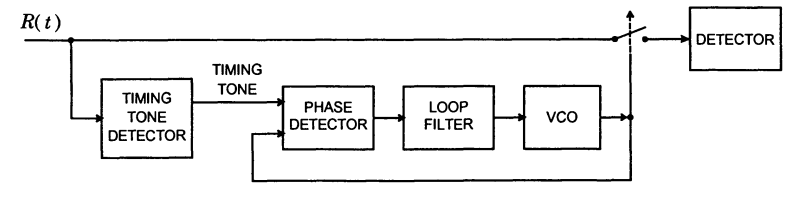
\includegraphics[width=.8\textwidth]{figs/metodo_dedutivo}
		\end{figure}
		\item Exemplo de método dedutivo: Método de linha espectral
		
	\end{itemize}			
\end{frame}

\begin{frame}
	\frametitle{Introdução - Recuperação de relógio}
	
	\begin{itemize}
		\item Método Indutivo: Não recupera o relógio diretamente do sinal recebido, mas através de um processo com \textit{feedback}
		\begin{figure}
			\centering
			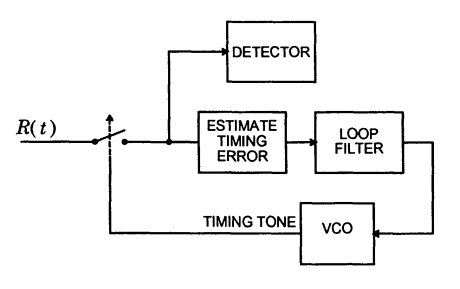
\includegraphics[width=.4\textwidth]{figs/metodo_indutivo}
		\end{figure}
		\item O método indutivo não utiliza o PLL como uma otimização opcional, PLL é parte integral do método
		\begin{itemize}
			\item Vantagem: boa parte da recuperação de relógio pode ser feita digitalmente e em tempo discreto
			\item Desvantagem: taxa de amostragem do sinal deve ser maior que a taxa de símbolo
			\item Exemplos: MMSE e suas aproximações
		\end{itemize}
	\end{itemize}			
\end{frame}

\section{Desempenho da recuperação de relógio}
% \subsection{Critérios de desempenho}

\begin{frame}
	\frametitle{Desempenho da recuperação de relógio}
% 	\framesubtitle{Critérios de desempenho}
	
	\begin{itemize}
		\item Além de saber a frequência de amostragem do sinal é importante saber onde amostrar (\textit{timing phase}).
		\item A sensibilidade do \textit{timing phase} pode ser analisada pelo diagrama de olho:
		
		\begin{columns}
			\begin{column}{.5\columnwidth}
				\begin{figure}
					\centering
					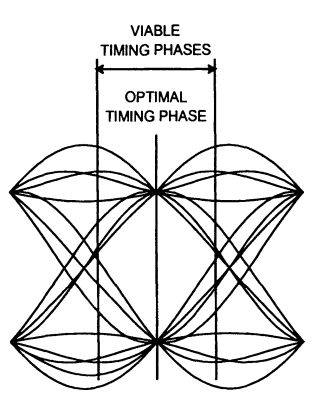
\includegraphics[width=.48\textwidth]{figs/olho_timing_phase_25}
				\end{figure}
			\begin{footnotesize} Pulso cosseno levantado (25\% roll-off) \end{footnotesize}
			\vspace{0.2cm}
			\end{column}
		~
		\begin{column}{.5\columnwidth}
			\begin{figure}
				\centering
				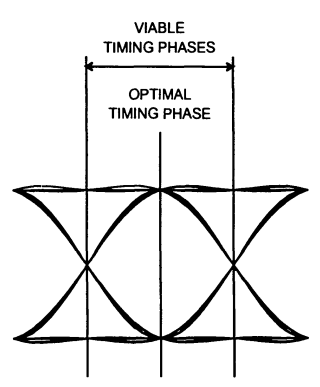
\includegraphics[width=.48\textwidth]{figs/olho_timing_phase_100}
				
			\end{figure}
		\begin{footnotesize} Pulso cosseno levantado (100\% roll-off) \end{footnotesize}
		\end{column}
		\end{columns}
		
		
	\end{itemize}			
\end{frame}


\begin{frame}
	\frametitle{Desempenho da recuperação de relógio}
% 	\framesubtitle{Critérios de desempenho}
	
	\begin{itemize}
		\item A recuperação do tom de tempo sempre sofrerá \textit{jitter} que pode ser reduzido a qualquer nível desejado.
		\begin{itemize}
			\item PLL ou projeto do circuito de recuperação.
		\end{itemize}
		\item Amostragem sub-ótima no ponto do olho aumenta a ISI e reduz a imunidade ao ruído.
		\item O fluxo de bit recuperado pelo detector sofrerá \textit{jitter} produzido pelo circuito de recuperação do relógio.
		\begin{itemize}
			\item Normalmente não é um grande problema para dados puramente digitais (ex: recebido por computadores).
			\item Problema quando representa um sinal contínuo no tempo (ex: áudio).
			\item Pode ser um problema em um sistema com repetidores.
		\end{itemize}
	\end{itemize}			
\end{frame}

\section{Métodos de linha espectral}

\begin{frame}
	\frametitle{Métodos de linha espectral}
% 	\framesubtitle{Métodos de linha espectral}
	
	\begin{itemize}
		\item Um sinal banda base PAM é ciclo-estacionário
		\begin{equation*}
		R(t) = \sum_{k=-\infty}^{\infty} A_kp\left(p-kT\right)
		\end{equation*}
		\item Seja um novo processo estocástico não linear e sem memória
		\begin{equation*}
		Z(t) = f\left(R(t)\right)
		\end{equation*}
		\item A esperança $E\left[Z(t)\right]$ é frequentemente não nula e periódica em $T$.
		\item O relógio pode ser recuperado passando $Z(t)$ através de um filtro banda passante centrado na taxa de transmissão (\textit{baud rate}).
	\end{itemize}			
\end{frame}

\begin{frame}
	\frametitle{Métodos de linha espectral linear}
% 	\framesubtitle{Métodos de linha espectral linear}
	
	\begin{itemize}
		\item Caso $E\left[R(t)\right]$ seja não nula, a forma de onda PAM contém linha espectral no \textit{baud rate}
		\begin{equation*}
		R(t) = E[A_k ]\sum_{m=-\infty}^{\infty} p\left(p - mT\right) + \sum_{m=-\infty}^{\infty}\left(A_m - E\left[A_k\right]\right)p\left(t-mT\right)
		\end{equation*}
		\item O primeiro termo é determinístico independente dos dados $A_k$ e possui periodicidade com período de $T$.
		\item O segundo termo possui média estocástica em zero.
		\item A periodicidade do primeiro termo tem o fundamental na taxa de símbolo $1/T$.
		\item Filtro banda passante pode recuperar o relógio (termo determinístico) com efeitos de \textit{jitter} (termo estocástico).
	\end{itemize}			
\end{frame}


\begin{frame}
	\frametitle{Métodos de linha espectral: exemplo}
% 	\framesubtitle{Métodos de linha espectral linear: exemplo}
	
	\begin{itemize}
		\item Considere um sinal binário \textit{on-off} com alfabeto $A_k\in \{0,1\}$ e um formato de pulso com $50\%$ de \textit{duty cycle} de um pulso quadrado
		\begin{equation*}
		p(t) = \begin{cases}
		1,& \text{for }t\in \left[ 0,T/2 \right) ,\\
		0,& \text{ caso contrário }
		\end{cases}
		\end{equation*}
		
		\begin{figure}
			\centering
			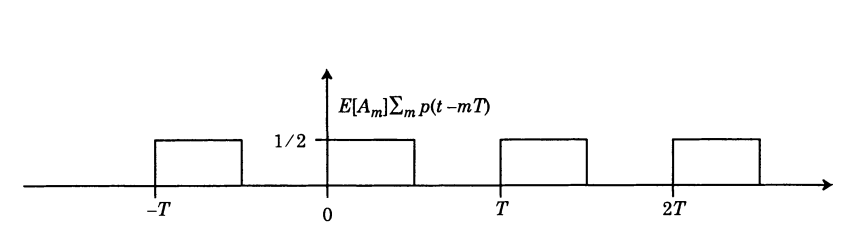
\includegraphics[width=.85\textwidth]{figs/on_off_pulse}
		\end{figure}
	\end{itemize}			
\end{frame}


\begin{frame}
	\frametitle{Métodos de linha espectral não linear}
% 	\framesubtitle{Métodos de linha espectral não linear}
	
	\begin{itemize}
		\item É possível que a média de $R(t)$ seja zero, mas momentos de ordem maiores podem ser diferentes de zero e periódicos.
			\item Por generalidade $A_k$ e $p(t)$ são valores complexos e processos brancos.
			\item A magnitude ao quadrado deste processo depende da função de correlação dos símbolos: $E[A_mA_n^*] = \sigma_A^2\delta_ {m-n}$
			\item Implicando em:
			\begin{equation*}
			E[|R(t)|^2] = \sigma_A^2\sum_{m=-\infty}^{\infty}|p(t-mT)|^2
			\end{equation*}
		\end{itemize}
		
		\begin{figure}
			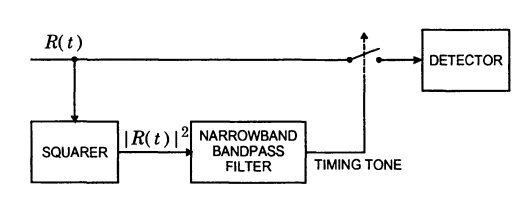
\includegraphics[width=0.5\textwidth]{figs/linha_espectral_nlinear}
		\end{figure}
\end{frame}

\begin{frame}
	\frametitle{Métodos de linha espectral não linear}
% 	\framesubtitle{Métodos de linha espectral não linear}
	\begin{block}{Exemplo de uma constelação binária antipodal}
		\begin{itemize}
			\item Considere um sinal em banda base, real, binário e antipodal $\{\pm a\}$
			\item A magnitude ao quadrado do sinal é dada por:
			\begin{equation*}
			R^2(t)= \sum_{m=-\infty}^{\infty} A_m^2p^2\left(t-mT\right) + \sum_{n}\sum_{m\neq n} A_nA_mp\left(t-nT\right)p\left(t-mT\right)
			\end{equation*}
		\end{itemize}

	\end{block}

\begin{itemize}
	\item Outros valores de potência também podem ser usados. Ex: $|R(t)|^4$
	\begin{itemize}
		\item $|R(t)|^4$ é eficiente com pouca largura de banda excedente.
		\item Em recuperação de portadora com sinal discreto de alta ordem podem ocasionar \textit{aliasing}.
	\end{itemize}
\end{itemize}
\end{frame}


\begin{frame}
	\frametitle{Métodos de linha espectral para sinais banda passante}
% 	\framesubtitle{Métodos de linha espectral para sinais banda passante}
	\begin{itemize}
		\item A metodologia de recuperação de relógio apresentada pode ser utilizada para PAM de banda passante após demodular o sinal
		\begin{itemize}
			\item Demodulação geralmente é aplicada após recuperação de relógio e equalização.
			\item Recuperação de portadora normalmente é feita usando o método "recuperação direcionada a decisão", o qual depende de um tempo de fase estável.
		\end{itemize}
		\item Com o método de linha espectral é possível recuperar o relógio sem demodular o sinal.
		\item Método chamado de derivação de relógio por envoltória.
	\end{itemize}
\end{frame}


\begin{frame}
	\frametitle{Métodos de linha espectral para sinais banda passante}
% 	\framesubtitle{Métodos de linha espectral para sinais banda passante}
	\begin{itemize}
		\item Relógio derivado da envoltória:
		\begin{itemize}
			\item Seja a saída de um filtro passa banda analítico:
			\begin{equation*}
			Y(t)=R(t)e^{j2\pi f_c t}
			\end{equation*}
			\item Em que $R(t)$ é um sinal banda base complexo. A magnitude deste sinal analítico é:
			\begin{equation*}
			|Y(t)|=|R(t)|\cdot |e^{j2\pi f_c t}| = |R(t)|
			\end{equation*}
			
			\item Calcular a magnitude ou magnitude ao quadrado é equivalente a aplicar um demodulador de sinal banda base.
			\item O receptor \textit{front-end} do receptor consiste em:
			\begin{itemize}
				\item Filtro banda passante, amostrador e separador de fase discreto.
				\item Amostrador deve ser controlado por um relógio (pode ser problemático).
			\end{itemize}
		\end{itemize}
		
	\end{itemize}
\end{frame}

\begin{frame}
	\frametitle{Métodos de linha espectral para sinais banda passante}
% 	\framesubtitle{Métodos de linha espectral para sinais banda passante}
	\begin{itemize}
		\item Relógio derivado da envoltória:
		\begin{itemize}
			\item Uma alternativa para usar o sinal analítico é utilizando $Re\{Y(t)\}$ (entrada do receptor)
			\begin{equation*}
			\left( Re\{Y(t)\} \right)^2 = \frac{1}{2}\left|Y(t)\right|^2 + \frac{1}{4}Y^2(t) + \frac{1}{4}\left(Y^*(t)\right)^2 \label{eq:real_signal}
			\end{equation*}
			\item Caso os símbolos $A_k$ sejam independentes, de média zero e os componentes reais e imaginários sejam independentes e possuam igual variância, temos:
			\begin{equation*}
			E[Re\{Y(t)\}^2] = \frac{1}{2}E[|Y(t)|^2]
			\end{equation*}
			
			\item  Função de recuperação do relógio é reduzida pela metade, aumentando o efeito do \textit{jitter}.
			\item Segundo e terceiro termos têm média zero, mas adicionam \textit{jitter}.
			
		\end{itemize}
		
	\end{itemize}
\end{frame}


\section{MMSE e aproximações}

\begin{frame}
	\frametitle{Método indutivo}
% 	\framesubtitle{Método indutivo}
	
	\begin{itemize}
		\item Método da linha espectral é popular mas nem sempre é possível realizar a recuperação de relógio no tempo contínuo.
		\item Exemplo:
		\begin{itemize}
			\item Cancelamento de eco (tempo discreto) deve ser realizado antes da recuperação de relógio.
			\item Conveniente recuperar relógio no tempo discreto.
		\end{itemize}
		\item Solução: recuperação de relógio por MMSE (método indutivo)
		\begin{itemize}
			\item Não é prático utilizando uma formulação exata.
			\item Há várias aproximações práticas que podem ser utilizadas.
		\end{itemize}
		
	\end{itemize}			
\end{frame}



\begin{frame}
	\frametitle{Algoritmo do gradiante estocástico}
% 	\framesubtitle{Algoritmo do gradiante estocástico}
	\begin{itemize}
		\item Recuperação de relógio por MMSE
		\begin{figure}
			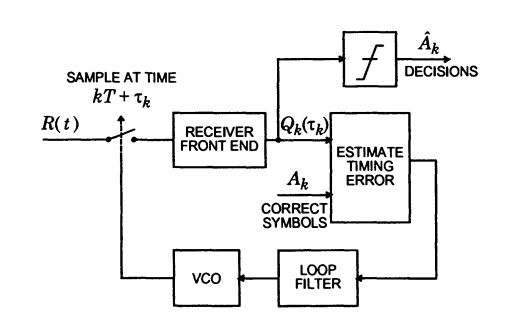
\includegraphics[width=.4\textwidth]{figs/mmse_timing_recovery}
		\end{figure}
		\item Objetivo é ajustar $\tau_k$ de forma a minimizar o erro médio quadrático:
		\begin{equation*}
		E[|E_k(\tau_k)|^2] =  E[|Q_k(\tau_k)-A_k| ]
		\end{equation*}
		
		\item É impossível achar uma solução fechada para minimizar o erro médio quadrático.
		\item É necessário um período de treinamento.
%		\item Podemos minimizar o erro quadrático médio atualizando $\tau_k$ iterativamente
	\end{itemize}			
\end{frame}

\begin{frame}
	\frametitle{Algoritmo do gradiante estocástico}
% 	\framesubtitle{Algoritmo do gradiante estocástico}
	\begin{itemize}
		\item Podemos minimizar o erro quadrático ajustando $\tau_k$ na direção oposta da derivada da esperança do erro quadrático médio
		\begin{equation*}
			\frac{\partial}{\partial \tau_k} E[|E_k(\tau_k)|^2] = E\left[\frac{\partial}{\partial\tau_k}|E_k(\tau_k)|^2\right]
		\end{equation*}
		\item $A_k$ não depende de $\tau_k$, então sabemos que:
		\begin{equation*}
		\frac{\partial E_k(\tau_k)}{\partial\tau_k} = \frac{\partial Q_k(\tau_k)}{\partial\tau_k} 
		\end{equation*}
%		\item E sabendo que:
%		\begin{equation*}
%	     \frac{\partial E_k(\tau_k)}{\partial\tau_k} = 2 Re \left\{ E_k^*(\tau_k) \frac{\partial E_k(\tau_k)}{\partial \tau_k} \right\}
%		\end{equation*}
		\item Iterativamente podemos ajustar $\tau_k$ através de:
		\begin{equation*}
		\tau_{k+1} = \tau_k - \alpha Re \left\{ E_k^*(\tau_k) \frac{\partial Q_k(\tau_k)}{\partial \tau_k} \right\}
		\end{equation*}
	\end{itemize}			
\end{frame}

\begin{frame}
	\frametitle{Algoritmo do gradiante estocástico}
% 	\framesubtitle{Algoritmo do gradiante estocástico}
	\begin{itemize}
		\item $Q_k(\tau_k)$ consistem em amostras de um sinal contínuo no tempo $Q(t)$ em que $t = kT+\tau_k$, então:
		\begin{equation*}
		\frac{\partial Q_k(\tau_k)}{\partial \tau_k} = \left[\frac{\partial Q(t)}{\partial t}\right]_{t = kT + \tau_k}
		\end{equation*}
		\item Então a atualização de $\tau_k$ é equivalente a
		\begin{eqnarray*}
			\tau_{k+1} & = & \tau_k -\alpha Re\left\{ E_k^*(\tau_k) \left[\frac{\partial Q(t)}{\partial t}\right]_{t = kT+\tau_k}\right\} \\
			& = & \tau_k -\alpha Re\left\{ \left[Q_k(\tau_k) - A_k\right]^* \left[\frac{\partial Q(t)}{\partial t}\right]_{t = kT+\tau_k}\right\}
		\end{eqnarray*}
	\end{itemize}			
\end{frame}


\begin{frame}
	\frametitle{Algoritmo do gradiante estocástico}
% 	\framesubtitle{Algoritmo do gradiante estocástico}
	\begin{itemize}
		\item O Algoritmo do gradiante estocástico não cumpre o objetivo de utilizar apenas amostras do sinal recebido
		\begin{itemize}
			\item Precisamos de $\frac{\partial Q(t)}{\partial t}$ (contínuo)
		\end{itemize}
	\item Sabemos que $Q_k(\tau) = Q(kT+\tau)$ e que $\tau$ varia lentamente ao ponto de considerarmos constante.
	\item Considerando que $Q(t)$ pode ser amostrado na taxa de Nyquist, podemos interpolar $Q_k(\tau)$
	\begin{equation*}
	Q(t) = \sum_{m=-\infty}^{\infty}Q_m(\tau) \frac{\sin [\pi (t-\tau-mT) ]/T}{\left[\pi (t-\tau-mT)\right]/T}
	\end{equation*}
	\end{itemize}
\end{frame}


\begin{frame}
	\frametitle{Algoritmo do gradiante estocástico}
% 	\framesubtitle{Algoritmo do gradiante estocástico}
	\begin{itemize}
		\item \begin{small} Assumindo a taxa de amostragem de Nyquist para $Q(t)$ pode-se  aproximar: \end{small}	
	\end{itemize}
	
	\begin{columns}
		\begin{column}{0.5\columnwidth}
			\begin{equation*}
			\frac{\partial Q_k(\tau_k)}{\partial \tau_k} = Q_k(\tau_k) * d_k
			\end{equation*}
		\end{column}
		~
		\begin{column}{0.5\columnwidth}
			\begin{equation*}
			d_k = \begin{cases}
			0 , & k=0\\
			\frac{(-1)^k}{kT}, & k \neq 0
			\end{cases}
			\end{equation*}
		\end{column}
	\end{columns}
	
	\begin{columns}
		\begin{column}{0.5\columnwidth}
			\begin{equation*}
			d_k  \approx \frac{\delta_{k+1}-\delta_{k-1}}{T}
			\end{equation*}
		\end{column}
		~
		\begin{column}{0.5\columnwidth}
			\begin{figure}
				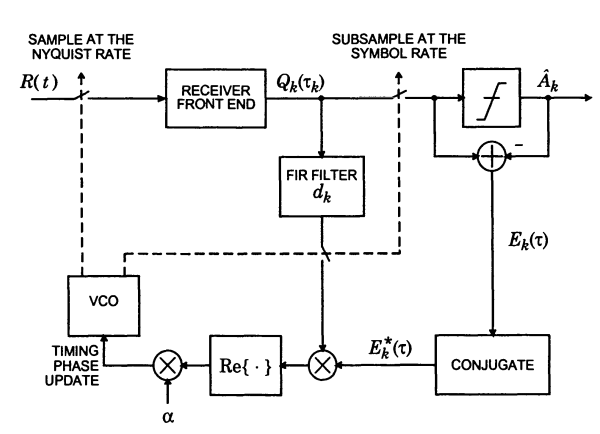
\includegraphics[width=\textwidth]{figs/aproximacao_gradiente}
			\end{figure}
		\end{column}
	\end{columns}
		
\end{frame}

\begin{frame}
	\frametitle{Algoritmo do gradiante estocástico}

	\begin{itemize}
		\item Com estas devidas aproximações teremos:
		\begin{equation*}
		\tau_{k+1} =  \tau_k -\alpha Re\left\{   [Q_k(\tau_k) - \hat{A}_k][Q_{k+1}(\tau_k) - Q_{k-1}(\tau_k)] \right\}
		\end{equation*}
		
	\end{itemize}
\end{frame}
